% Manuscript for Computational Materials Science (elsarticle, numbered refs).
\documentclass[preprint,12pt]{elsarticle}

\usepackage{amsmath,amssymb}
\usepackage{graphicx}
\ifx\pdfmapfile\undefined\else\pdfmapfile{+cm-super-t1.map}\fi % Type 1 EC fonts
% file names in Data availability break at underscores instead of overflowing
\usepackage{url}
% Let TeX use an extra pass on the few paragraphs that would otherwise
% overflow the measure (long unbreakable formulae and compounds).
\setlength{\emergencystretch}{1em}
% hyperref omitted: Elsevier typesets the accepted manuscript itself

% ---------------------------------------------------------------

\begin{document}

\begin{frontmatter}

\title{Atomistic bounds on the magnetostrictive mechanism of magnetic-memory
plasticity in Al--Mg--Si alloys with iron-bearing inclusions}

\author[mospolytech]{I.~Mikhailovskiy\corref{cor1}}
\ead{ilyamihailovsy@gmail.com}
\author[mospolytech]{D.~Pshonkin}
\cortext[cor1]{Corresponding author.}
\affiliation[mospolytech]{organization={Moscow Polytechnic University},
  city={Moscow}, country={Russia}}

\begin{abstract}
How pre-exposing an Al--Mg--Si alloy with Al$_{13}$Fe$_4$ inclusions to a
static magnetic field affects plastic deformation in creep is
examined by molecular dynamics. The inclusion is elongated along the field by
0.194\%, the strain corresponding to the 147~MPa interface stress estimated
experimentally, and is held at that strain while the matrix relaxes. The
resolved shear stress in the matrix reaches 15~MPa above the inclusion
and falls to the resolution of the calculation within 80~\AA{}.
Under shear, a pre-existing dislocation pair is torn apart from 95--105~MPa,
and no new dislocation forms at the interface up to 400~MPa in the unstrained
cell. A two-scale estimate reproduces the measured 25\% creep increase for the activation volumes reported for Al--Mg--Si,
provided the inclusions strain by 0.194\%; the magnetostriction measured for
Fe--Al is twenty times smaller, and the persistence of the effect after the
field is removed is not explained by an elastic stress.
\end{abstract}

\begin{keyword}
magnetoplasticity \sep magnetic memory \sep creep \sep molecular dynamics
\sep Al--Mg--Si alloys \sep Al$_{13}$Fe$_4$ \sep interface stress \sep
dislocations \sep solute pinning
\end{keyword}

\end{frontmatter}

\section{Introduction}
\label{sec:intro}

Weak magnetic fields, whose energy per atom is negligible compared with the
thermal energy $kT$, nevertheless change the plasticity of nonmagnetic
crystals; the broad class of such observations is known as the magnetoplastic
effect \cite{Alshits2003,Molotskii2000}. Aluminum alloys with Fe-bearing
inclusions occupy a special place in this class because, if such an inclusion
is ferromagnetic, they offer a seemingly straightforward mechanical route from
the field to plastic flow: the field magnetizes the inclusion;
magnetostriction---the change of shape that a magnetized body
undergoes---strains it; and the stress caused by the mismatch between the
strained inclusion and the surrounding matrix is transferred to the matrix.
Whether the inclusions in these alloys are in fact ferromagnetic is considered
in Section~\ref{sec:phase}. A series of experiments on a commercial
Al--Mg--Si alloy with iron-bearing microinclusions has documented the effect
in detail: a 30~min exposure to $B=0.4$--$0.7$~T, applied \emph{before}
mechanical testing, increases the subsequent room-temperature creep
strain---the slow deformation under a constant load---at 160~MPa by roughly a
quarter, increases the heat release during deformation several-fold, and
shifts the Taylor--Quinney coefficient, the fraction of the work of plastic
deformation that is released as heat, from 0.07 to 0.25
\cite{Skvortsov2019JAP,Skvortsov2019PSS,Friha2024JMMM,Nikolaev2025SciRep}.
Because the effect remains after the field is removed, it has been described
as ``magnetic memory'' in plasticity \cite{Skvortsov2019PSS}.

The interpretation advanced in these works rests on a single estimate. The
stress at the inclusion--matrix interface produced by magnetostriction of the
inclusion, obtained from the field strength through an empirical
proportionality coefficient, is put at about 147~MPa for $B=0.7$~T
\cite{Friha2024JMMM}. This exceeds the 120~MPa yield stress of the matrix,
and the conclusion drawn is that the matrix around every inclusion is
plastically deformed and its density of dislocations---the line defects of
the crystal lattice whose motion produces plastic flow---is raised. This chain
of reasoning has never been examined at the scale on which it is supposed to
act. Whether a stress of this magnitude actually appears in the matrix, over
what distance from the interface it persists, and whether it is capable of
nucleating dislocations or of setting existing ones in motion are questions
about {\aa}ngstr{\"o}ms and picoseconds---the native domain of classical
molecular dynamics (MD), in which the atoms move according to Newton's
equations under forces derived from an interatomic potential.

In the present work the magnetostrictive mechanism is subjected to a
quantitative atomistic test at the interface between aluminum and the
intermetallic compound Al$_{13}$Fe$_4$. A magnetic field has no direct
representation in classical MD, so its action is represented mechanically:
based on the earlier experimental work \cite{Friha2024JMMM}, the inclusion
is taken to elongate along the field direction by
$\varepsilon=1.94\times10^{-3}$ (0.194\%) at constant volume, the strain
corresponding to the 147~MPa interface stress estimated there. A direct
reproduction of the macroscopic effect in a simulation cell is not attempted;
the reason is set out in Section~\ref{sec:discussion}. Instead, each link of
the proposed chain is examined separately. The following quantities are
computed: the stress field that the elongated inclusion creates in the matrix
and its decay with distance from the interface; the applied shear stress at
which a dislocation already present in the matrix starts to move, and that
and whether new dislocations are nucleated at the interface up to the highest stress applied; and the resistance
that Mg and Si solute atoms dissolved in the aluminum oppose to dislocation
motion. The chain is then closed from the opposite end: a two-scale estimate
gives the interface stress that the measured 25\% creep enhancement
\emph{requires}, assuming thermally activated glide---dislocation motion in
which obstacles are overcome with the help of thermal fluctuations, so that
the glide rate depends exponentially on the stress---and the decay as
$r^{-3}$ of the elastic field outside a strained inclusion
\cite{Eshelby1957}.

\section{Computational methods}
\label{sec:methods}

\subsection{Interface cell}
\label{sec:cell}

All calculations were performed with LAMMPS (22~Jul~2025 release, KOKKOS/CUDA
build for graphics processors) \cite{Thompson2022LAMMPS}. Interatomic forces
are given by the 2NN-MEAM potential (second-nearest-neighbour modified
embedded-atom method) of Jelinek \emph{et al.} for the Al--Si--Mg--Cu--Fe
system \cite{Jelinek2012}, a single potential that describes every atom in
the cell, including the atoms on either side of the interface, by one set of
interaction rules.

The matrix is face-centred cubic (fcc) aluminium ($a=4.05$~\AA{}). Its
orientation, $x\parallel[1\bar{1}0]$, $y\parallel[11\bar{2}]$,
$z\parallel[111]$, is dictated by the slip system of fcc Al: dislocations in
aluminium move on $\{111\}$ planes along $\langle110\rangle$ directions, and
with this choice the (111) glide plane is parallel to the interface and the
$[1\bar{1}0]$ glide direction lies along $x$. An edge dislocation (the edge
of an extra half-plane of atoms inserted into the crystal) with Burgers
vector $\tfrac{1}{2}[1\bar{1}0]$---the lattice translation that measures the
displacement it carries, $|\mathbf{b}|=2.86$~\AA{}---and line along $y$ then spans the whole width of the cell, so that it
represents an infinitely long straight dislocation, and glides in $x$
parallel to the interface,
which is the motion the mechanism under test would have to produce.

The inclusion is the monoclinic intermetallic Al$_{13}$Fe$_4$ in the
structure of Ref.~\cite{Liu2024CIF}. It is built as a flat layer 20~\AA{}
thick that carries on its upper surface a half-elliptical bulge (referred to
below as the ridge) with semi-axes 35~\AA{} along $x$ and 20~\AA{} along $z$,
running the full length of the cell along $y$. The ridge is essential: a
flat strained layer that spans the entire cell can relieve its normal stress
simply by expanding upward, and it is the curved edges of the ridge that
produce a non-uniform stress field in the matrix, as the curvature of the
surface of a real particle would. The flat layer is left unstrained and the ridge alone carries the strain
(Section~\ref{sec:eigenstrain}).

In $x$ and $y$ the cell is periodic: an atom leaving through one face
re-enters through the opposite face, so the cell represents an interface
unbounded in its plane. The in-plane dimensions ($L_x=154.64$~\AA{}, $L_y=64.48$~\AA{}: 54 and 13
periods of the aluminium lattice, ten and eight cells of Al$_{13}$Fe$_4$) are
chosen so that both lattices are periodic in the plane. The small residual
mismatch ($-0.22\%$ along $x$, $-0.26\%$ along $y$) is taken up by the
inclusion and is the same in the strained and in the control cell, so that it
cancels to first order when the two are compared. Aluminium atoms lying within
2.2~\AA{} of an inclusion atom (periodic images included) are removed; the
smallest interatomic distance in the resulting structure is 2.22~\AA{}. The
aluminium layer above the interface plane is 129~\AA{} thick (56 atomic (111)
planes), the whole cell contains 91\,428 atoms (72\,532 in the matrix and
18\,896 in the inclusion), and in $z$ it is bounded by a free surface with
17~\AA{} of vacuum above it and by a layer 6~\AA{} thick at the bottom whose
atoms are held fixed (Fig.~\ref{fig:cell}).

The inclusion is bonded to the matrix. Atoms on both sides of the interface
interact through the same potential, no constraint or artificial coupling is
imposed at the interface, and the interface neither slips nor opens except
through the atomic displacements the potential itself allows. The control structure is relaxed in three stages: energy minimisation by
conjugate gradients (the atoms are moved to positions of minimum energy
without thermal motion), 6~ps of molecular dynamics at 300~K followed by
12~ps of cooling to 0.5~K, which relax the long-wavelength modes of the slab
that minimisation alone does not reach, and a final minimisation to a force
of 0.05~eV/\AA{} (two-norm over all atoms). The strained cell is built from
this relaxed state (Section~\ref{sec:eigenstrain}) and minimised to
0.02~eV/\AA{}.

\begin{figure}
\centering
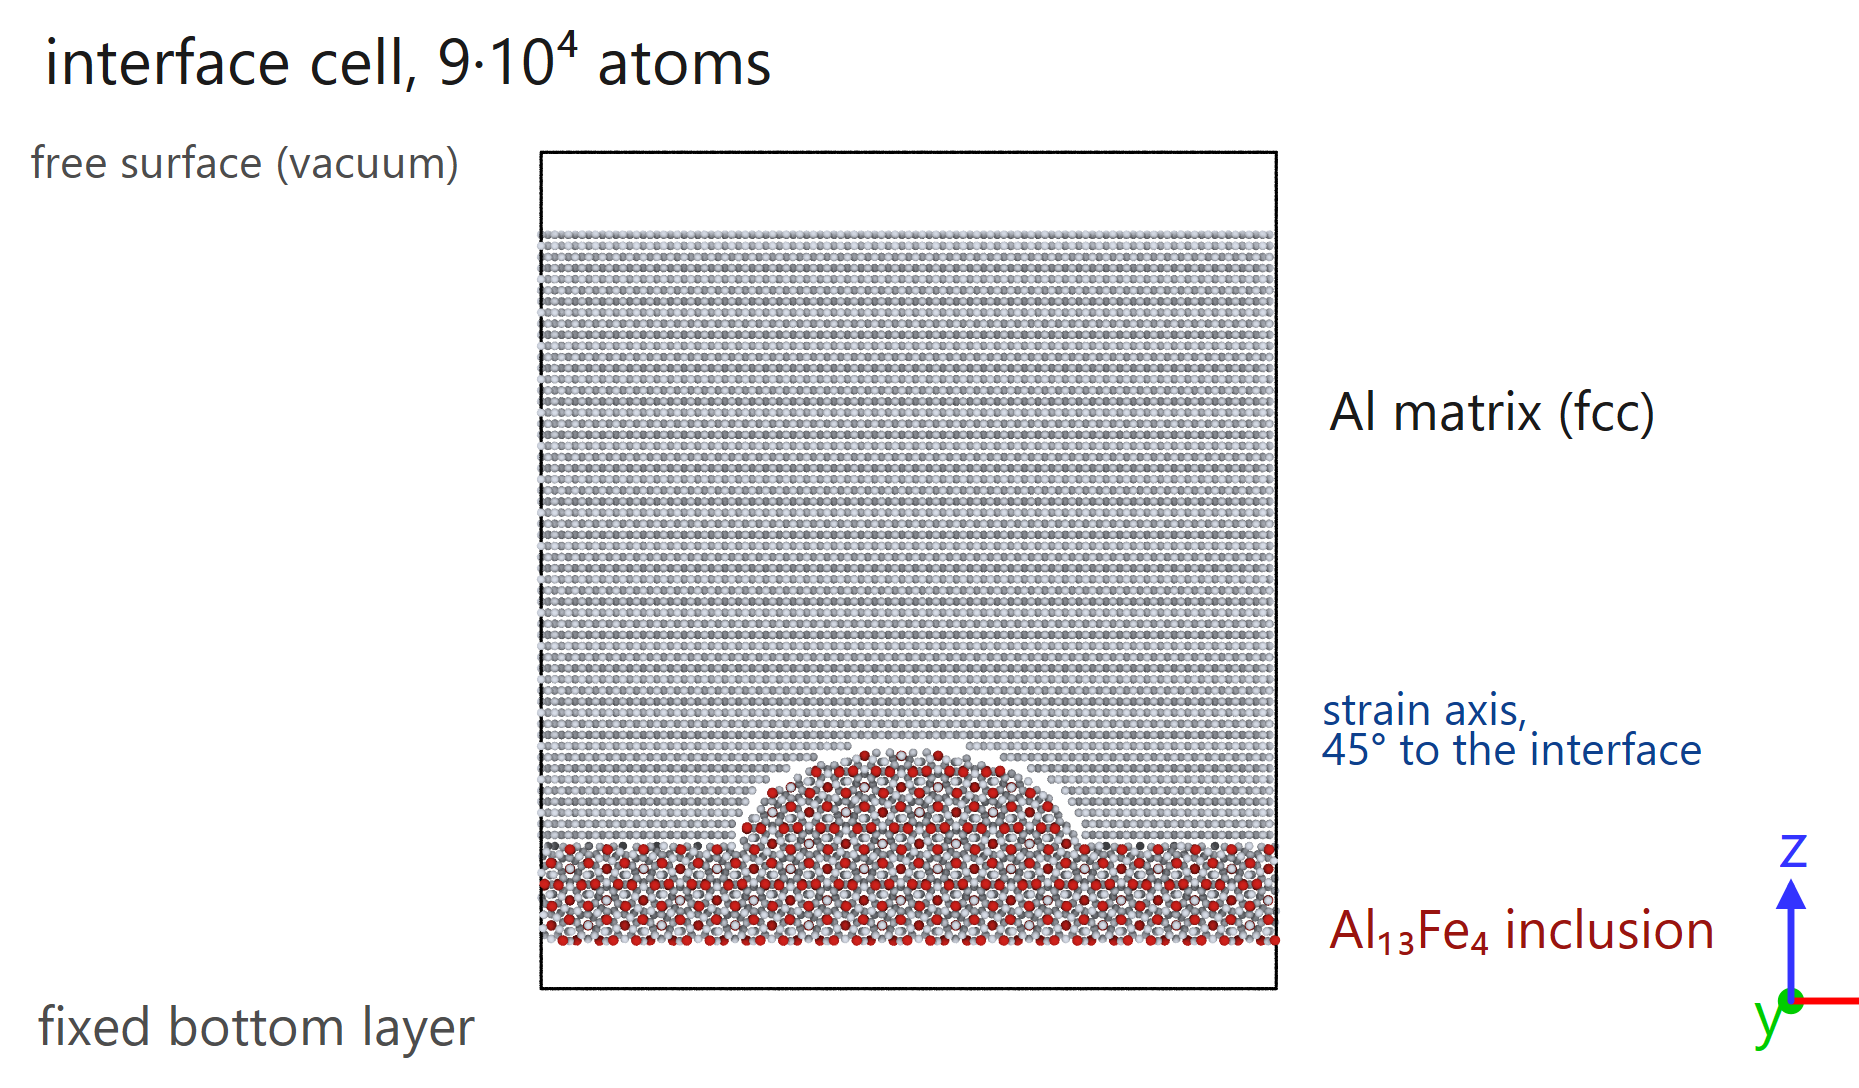
\includegraphics[width=0.92\linewidth]{fig_cell_interface_en}
\caption{The interface cell, viewed along $y$ (the $x$--$z$ plane). Grey:
the aluminium matrix, 129~\AA{} of fcc aluminium with $x=[1\bar{1}0]$,
$y=[11\bar{2}]$ and $z=[111]$, so that the interface is parallel to a (111)
glide plane and $x$ is a glide direction. Red: the Al$_{13}$Fe$_4$ inclusion,
a flat layer with a half-elliptical ridge 70~\AA{} wide and 20~\AA{} high.
The lowest 6~\AA{} of the inclusion are held fixed; above the aluminium is
vacuum. The cell is periodic along $x$ and $y$. The imposed elongation of the
inclusion is directed at $45^{\circ}$ to the interface in the $x$--$z$
plane.}
\label{fig:cell}
\end{figure}

\subsection{Representation of the field}
\label{sec:eigenstrain}

Molecular dynamics is classical mechanics, and the magnetic field itself is
not present in the calculation. Its action is represented mechanically, by
the strain it is assumed to produce in the inclusion. Following the earlier
experimental studies
\cite{Skvortsov2019JAP,Skvortsov2019PSS,Friha2024JMMM,Nikolaev2025SciRep},
in which the field acts through magnetostriction, i.e. the elongation of the
inclusion along the direction of the field, the inclusion is taken to
elongate along the field direction $\mathbf{u}$ by
$\varepsilon=1.94\times10^{-3}$ (0.194\%), the elastic strain
$\sigma_m/E_{\mathrm{Al}}$ (with $E_{\mathrm{Al}}=75.7$~GPa) corresponding to
the interface stress $\sigma_m=147$~MPa estimated in those works
\cite{Friha2024JMMM}, at constant volume: elongation $\varepsilon$ along $\mathbf{u}$ and contraction
$\varepsilon/2$ along the two perpendicular directions. Written as a tensor,
\begin{equation}
\varepsilon^{*}_{ij}
  =\tfrac{3}{2}\,\varepsilon\!\left(u_i u_j-\tfrac{1}{3}\delta_{ij}\right),
\qquad \operatorname{tr}\varepsilon^{*}=0,
\label{eq:eigenstrain}
\end{equation}
where $\delta_{ij}$ equals 1 for $i=j$ and 0 otherwise and the zero trace
expresses the constancy of volume. In the elasticity of inclusions a strain
of this kind, the one the inclusion would adopt if it were free of the
matrix, is called an eigenstrain \cite{Eshelby1957}; the term is used below
in that sense. The value adopted is well above the magnetostriction measured
in Fe--Al alloys \cite{Hall1959,BormioNunes2012}; it is used because it is
the amplitude the proposed mechanism itself presupposes, and the mechanism
is tested at that amplitude.

The direction $\mathbf{u}$ is inclined at $45^{\circ}$ to the interface
normal, in the $x$--$z$ plane. The reason is geometric. For $\mathbf{u}$
along the normal $z$ the imposed strain produces no shear stress at all on
the $(111)[1\bar{1}0]$ glide system: the Schmid factor (the geometric factor
that converts a stress into the shear stress acting on a given slip system)
is exactly zero, and no force whatever would act on a dislocation gliding
parallel to the interface. At $45^{\circ}$ the shear component of the
imposed strain on the glide plane is at its maximum,
$\varepsilon^{*}_{xz}=\tfrac{3}{4}\varepsilon=1.46\times10^{-3}$. In a
polycrystal the grains that respond to the field are those whose slip planes
are favourably inclined to it, and the tilted cell represents that
population. The tilt is the same in every cell.

The strain is applied by displacing every atom of the ridge relative to the
centre of the ridge in proportion to its position,
$\mathbf{r}\rightarrow\mathbf{r}+\varepsilon^{*}\!\cdot\!\mathbf{r}$, which
stretches the ridge uniformly along $\mathbf{u}$ and compresses it across
$\mathbf{u}$. The flat layer beneath the ridge is left unstrained. It spans
the periodic cell, and a layer that is periodic in its plane cannot be
sheared coherently: held at the shear of Eq.~(\ref{eq:eigenstrain}) its
surface would be a sawtooth with a step of $\varepsilon^{*}_{xz}L_x=0.22$~\AA{}
at the cell boundary, and the whole aluminium slab above it would be
stretched along $z$ by about $\varepsilon^{*}_{xz}$---a stress of order
150~MPa across the cell, which is what was observed when this was tried. The
ridge is the particle whose field is measured; the layer only closes the
cell. The interatomic potential is not modified. The stress field
produced by the strained inclusion is obtained as the difference between a
cell with the strained inclusion and a control cell without strain, both
minimised from identical starting structures under identical conditions. Two
variants are computed, differing in whether the inclusion is allowed to
relax.

In the \emph{maintained} case every inclusion atom---the ridge at its
displaced position, the flat layer at its original one---is held by a stiff
spring (stiffness 20~eV/\AA$^{2}$, which keeps the atom within about
0.01~\AA{} of that position) while the matrix relaxes around it, so that the
ridge holds the strain of Eq.~(\ref{eq:eigenstrain}) throughout. The springs
are attached in the same way in the corresponding control cell, so they
cancel in the difference between the two. This cell gives the stress field
of a particle that maintains its eigenstrain.
Under the forces that arise at the interface the inclusion atoms depart from
their strained positions by about 0.01~\AA{}, and the ridge retains
$0.97\pm0.004$ of the imposed strain (measured as described for the free case
below).

In the \emph{free} case no springs are attached and the inclusion is free to
relax the imposed strain back out. It does so to a large extent: after
minimisation the ridge, which produces the field measured in the matrix,
retains 0.2--0.4 of the imposed strain ($0.20\pm0.11$ and $0.44\pm0.10$ in
two minimisations, both stopped before full convergence). The fraction is measured as the
projection of the residual distortion of the Fe sublattice of the inclusion
onto $\varepsilon^{*}$, obtained by a least-squares fit of the displacements
between the strained and the control cell; the uncertainty is the standard
error of that fit. The free cell shows what an inclusion does when nothing
holds its strain; its stress field is the relaxed response, not the field of
an inclusion that maintains the strain, and it is the maintained case that is
compared with the dislocation thresholds below.

The \emph{control} cell has no strain. It is the relaxed structure of
Section~\ref{sec:cell} itself; the strained cell is built from it, minimised
with the same tolerance and compared with it atom by atom, so that the
residual lattice mismatch of Section~\ref{sec:cell}, the arrangement of the
interfacial layer and the long-wavelength strain of the slab are common to
both and cancel in the difference. The interface cells supply the stress profile in the
matrix and its decay length. The stresses at which dislocations begin to move
are obtained separately, in the loaded cells of Section~\ref{sec:loading},
and serve only as the thresholds against which that profile is compared.

\subsection{Loaded cells and loading scheme}
\label{sec:loading}

The stresses at which dislocations move are measured in two cells loaded in
shear under dynamics at 300~K.

The first is the interface cell of Section~\ref{sec:cell} with a
pre-existing pair of edge dislocations placed next to the ridge of the
inclusion, 91\,428 atoms in all (Fig.~\ref{fig:loading}). The pair is
a dislocation dipole: two parallel dislocations of opposite sign whose stress
fields attract, so that in a uniform, stress-free crystal the pair is stable and stays where it is placed until
the applied stress exceeds the level at which the two partners can pass each
other. Both dislocations lie along $y$ and glide on (111) planes parallel to
the interface. The partners are offset by 23.4~\AA{} along $x$ and by ten
(111) interplanar spacings, 23.4~\AA{}, along $z$, so that the line joining
them is inclined at $45^{\circ}$ to the glide planes. Two edge dislocations
of opposite sign on glide planes a distance $h$ apart attract with a shear
stress of up to $\mu b/[8\pi(1-\nu)h]$, which for $h=23.4$~\AA{} is 198~MPa
(with $\mu=26.5$~GPa, $\nu=0.347$ and $b=2.864$~\AA{}); this is the applied
stress at which they would pass each other in an unbounded crystal. The lower
partner is placed 27~\AA{} beyond the foot of the ridge and 29~\AA{} above the
interface plane, the upper one 23~\AA{} higher and 23~\AA{} closer to the
ridge. The cell is loaded by a shear stress raised
linearly from 0 to 400~MPa over 96~ps, after 5~ps at zero stress. The stress
is applied as a uniform force along $x$ on the atoms of the top atomic
layers, with the reaction taken by the fixed bottom layer; the rate of rise
is switched on smoothly over the first 16~ps so that the lowest shear
vibration of the slab is not excited. The loading is far faster than any
laboratory test (an effective strain rate of order $10^{8}$~s$^{-1}$), so the
thresholds obtained are upper estimates relative to slow loading. Three ramps were run: the unstrained cell with the inclusion free to relax,
to 400~MPa over 96~ps; and the unstrained and the strained cell with the
inclusion held by the springs of Section~\ref{sec:eigenstrain}, at the same
rate of rise, to 145~MPa over 40~ps---the pair that compares strained with
unstrained.

The second cell has no inclusion. It is a slab of the alloy matrix with the
same orientation, 92\,800 atoms (91\,315~Al, 928~Mg, 557~Si; $114.6\times49.6\times291$~\AA{}), in which
1.0~at.\%~Mg and 0.6~at.\%~Si are placed at random on lattice sites, and
which contains one edge dipole whose partners lie 206~\AA{} apart on parallel
glide planes; their mutual attraction corresponds to a shear stress
$\mu b/[8\pi(1-\nu)h]\approx22$~MPa, small compared with the stresses
applied. Before loading, the structure is energy-minimised and brought to
300~K. This cell is loaded in steps: constant shear stresses of 45, 55, 65
and 75~MPa, each held for 30~ps and each switched on smoothly over 4~ps,
after 10~ps at zero stress. Steps are used rather than a ramp because a
dislocation held by solute atoms moves by breaking away from them, a
thermally activated event whose waiting time depends on the stress; holding
the stress constant for a fixed time tests whether the dislocation breaks
away at that level, and the stress is raised in steps to find the level at
which it does. A pure-aluminium cell of the same geometry provides the
solute-free reference.

In both cells the equations of motion are integrated with a time step of
1~fs, about a hundredth of the period of an atomic vibration. The temperature
is held at 300~K by a Nos\'e--Hoover thermostat (damping time 0.1~ps), which
keeps the average kinetic energy of the unconstrained atoms at the set value
by a weak feedback on their velocities. The dislocations are inserted by the
Volterra construction, in which the crystal is cut along a half-plane, the
two faces are displaced relative to each other by one Burgers vector and
rejoined, with the displacement field made compatible with the periodic
cell. The dislocation content of every starting structure is verified with
the dislocation extraction algorithm (DXA) \cite{Stukowski2012DXA}, which
locates dislocation lines in an atomic configuration and determines their
Burgers vectors, as implemented in OVITO \cite{Stukowski2010OVITO}.

\begin{figure}
\centering
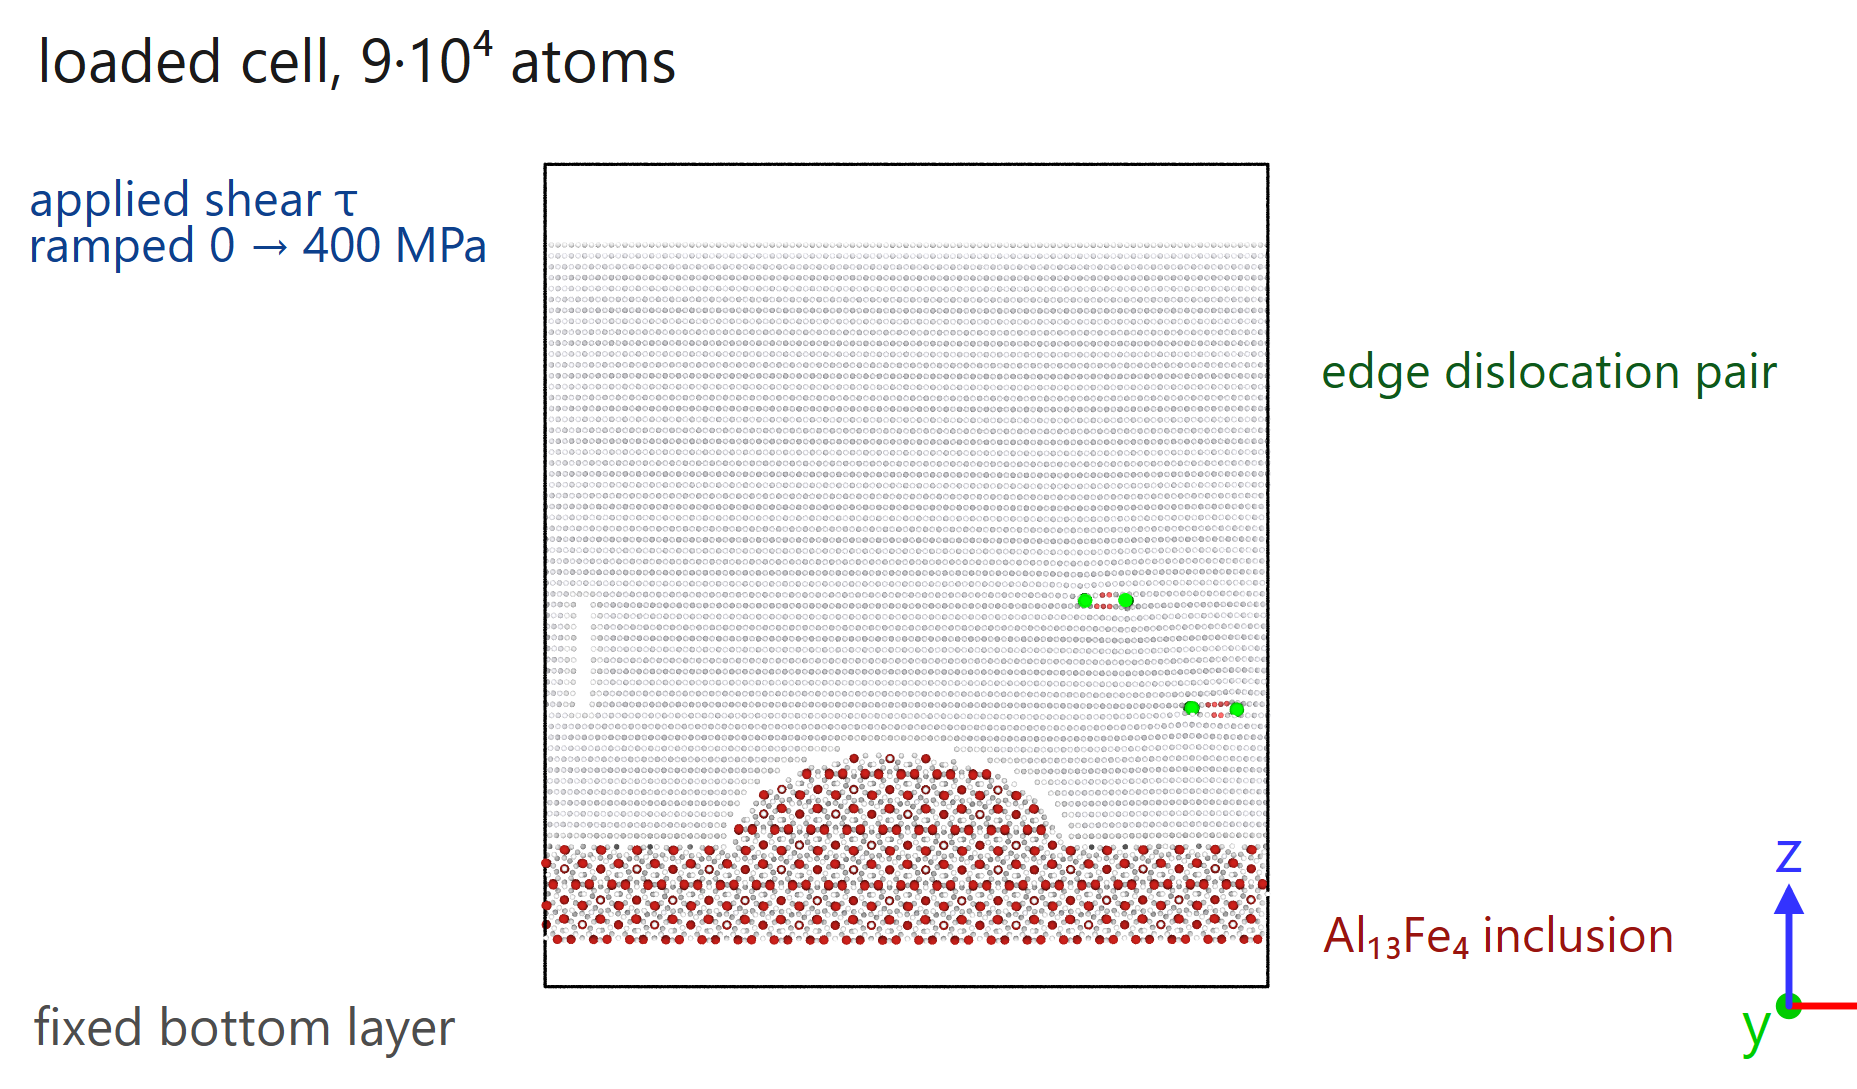
\includegraphics[width=0.92\linewidth]{fig_cell_loading_en}\\[2mm]
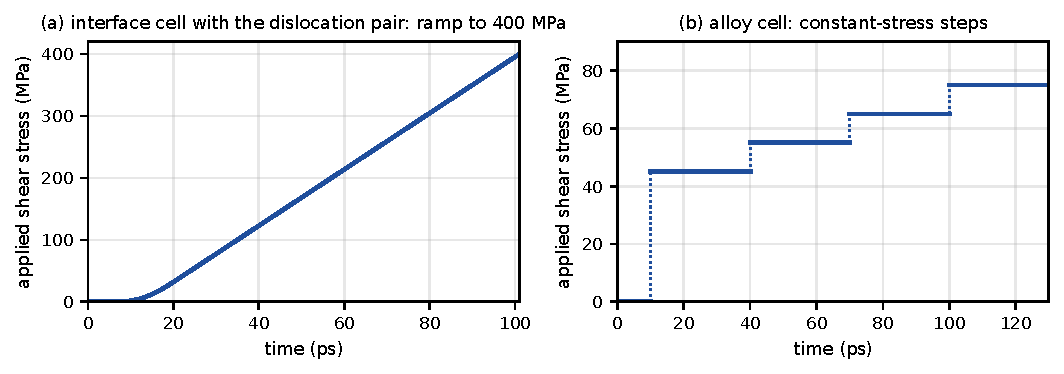
\includegraphics[width=0.92\linewidth]{fig_loading_programme_en}
\caption{The loaded interface cell (top) and the two loading programmes
(bottom). Top: the cell of Fig.~\ref{fig:cell} with a pair of edge
dislocations of opposite sign next to the ridge (green: the dislocation lines
found by dislocation analysis; atoms of the perfect lattice are faded), both
on (111) glide planes parallel to the interface. A shear stress $\tau$ along
$x$ is applied through a uniform force on the top atomic layers and is taken
up by the fixed bottom layer. Bottom: the stress programmes---for this cell a
linear rise from 0 to 400~MPa over 96~ps after 5~ps at zero stress (the
held cells were ramped at the same rate to 145~MPa) (a); for
the alloy cell without inclusion (Section~\ref{sec:mobility}) steps of 45,
55, 65 and 75~MPa, 30~ps each, after 10~ps without load (b).}
\label{fig:loading}
\end{figure}

\subsection{Stress evaluation}
\label{sec:stress}

Local stresses are obtained from the per-atom virial stress, the atomic-scale
counterpart of mechanical stress, computed for each atom from the forces
between it and its neighbours and divided by the atomic volume
$\Omega=16.61$~\AA$^{3}$: $\sigma_{ij}=-\langle W_{ij}\rangle/\Omega$. The
stress of a single atom fluctuates thermally by several GPa, so no scalar
measure is ever formed atom by atom. The six components of the tensor are
first averaged over a slice 4~\AA{} thick parallel to the interface (and, in
the dynamic runs, over time frames), and only then are two scalar measures
formed from the averaged tensor: the von Mises stress, a single positive number that measures the shear
content of a stress state and enters the yield criterion of a ductile metal,
and the resolved shear stress,
the shear stress acting on a given slip plane in a given slip direction.
$\mathrm{RSS}_{\max}$ denotes the largest resolved shear stress among the
twelve $\{111\}\langle110\rangle$ slip systems of the matrix, i.e. the shear
stress on the most favourably oriented system.

Stress profiles $\sigma(r)$ are built as functions of the distance $r$ from
the interface plane in slices 4~\AA{} thick, using only matrix atoms that lie
above the crest of the ridge, so that $r$ measures the distance from the
inclusion surface. The field of the strained inclusion is the difference
between the strained and the control cell, slice by slice. On energy-minimised
structures there is no thermal motion, and the noise level of that difference
is set by the residual slice-to-slice scatter far from the interface: over
$r\geq60$~\AA{} the mean of $\Delta\mathrm{RSS}_{\max}$ is $2.5\pm0.5$~MPa
(mean and standard deviation over thirteen slices), the resolution of the
calculation, below which no field is resolved.

\section{Results}
\label{sec:results}

\subsection{The interface stress field and its decay}
\label{sec:sigma_r}

Figure~\ref{fig:sigma} shows how the stress in the aluminium matrix varies
with the distance $r$ from the interface plane in the two interface cells of
Section~\ref{sec:cell}: the control cell, in which the ridge is unstrained,
and the cell in which the ridge has been elongated by
$\varepsilon=1.94\times10^{-3}$ along the field direction and held there
(Section~\ref{sec:eigenstrain}). The strained cell is built from the relaxed
control by displacing the ridge atoms and is then minimised, so that the two
cells differ in nothing but the strain of the ridge. The matrix is cut into
slices 4~\AA{} thick parallel to the interface, the six components of the
stress tensor are averaged over the aluminium atoms of each slice, and only
then are invariants formed from the averaged tensor
(Section~\ref{sec:stress}). Two averages are used. The first spans the whole
cell in $x$ and $y$, i.e.\ the region above the ridge and the region beside
it; the second is restricted to a window 20~\AA{} wide centred on the ridge
axis, which is the stress that the matrix sees directly above the inclusion.
The ridge---the half-elliptic bump of the inclusion, with semi-axes 35~\AA{}
along $x$ and 20~\AA{} along $z$ (Fig.~\ref{fig:cell})---has its crest at
$r=20$~\AA{}, so that above the crest the distance to the nearest inclusion
surface is $d=r-20$~\AA{}.

\begin{figure}
\centering
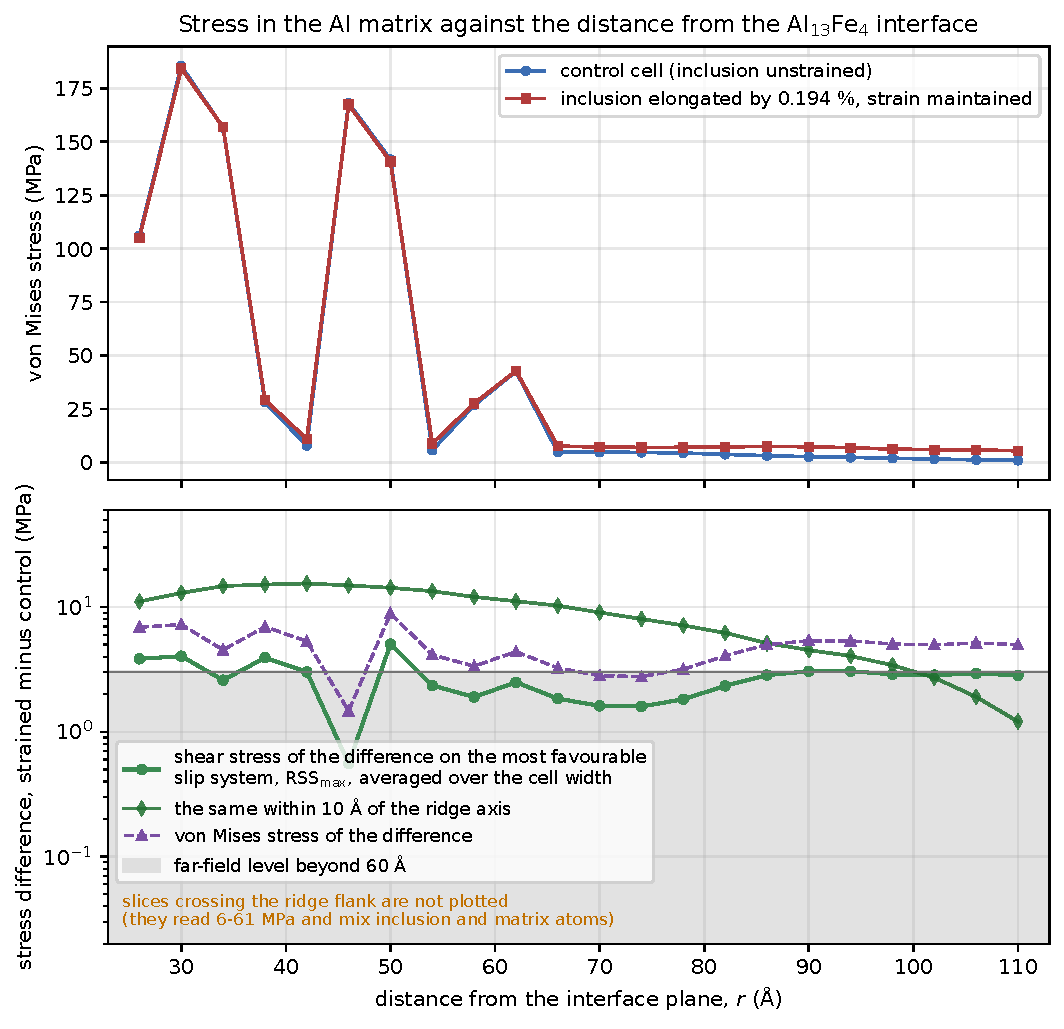
\includegraphics[width=0.85\linewidth]{fig_sigma_profile_en}
\caption{Stress in the aluminium matrix as a function of the distance $r$
from the interface plane in the two interface cells (91\,428 atoms): the
control cell with the unstrained ridge, and the cell in which the ridge is
elongated by 0.194\% along the field direction and held at that strain. The
matrix is cut into slices 4~\AA{} thick parallel to the interface; the six
stress components are averaged over the aluminium atoms of each slice before
any invariant is formed. Top: the von Mises stress in each cell; the
100--190~MPa just above the ridge crest, present in both cells, is the
coherency stress of the bonded interface between two crystals of different
spacing, and the curves coincide. Bottom: the difference
$\Delta\sigma_{ij}=\sigma_{ij}(\varepsilon)-\sigma_{ij}(0)$ as the shear
stress resolved onto the most favourable of the twelve slip systems of fcc
Al, $\mathrm{RSS}_{\max}$, averaged over the whole width of the cell
(circles) and within 10~\AA{} of the ridge axis (diamonds), together with
the von Mises stress of the difference tensor. The shaded region marks stresses below 3~MPa: the width-averaged level
beyond 60~\AA{} with its scatter, $2.5\pm0.5$~MPa, the resolution of the
calculation for long-wavelength strains of the slab. Slices at the level of
the ridge flanks, closer to the interface plane than the crest, are omitted:
there $r$ is not a distance to the inclusion surface and the slices contain
inclusion atoms. The profile ends 20~\AA{} below the free surface of the
slab.}
\label{fig:sigma}
\end{figure}

The upper panel gives the von Mises stress (Section~\ref{sec:stress}) in
each cell. Two features of the control curve need to
be stated plainly, because they are present without any imposed strain.
First, in the slices just above the ridge crest the stress is 100--190~MPa,
and at the level of the ridge flanks it reaches 0.8--2.2~GPa. This is the
coherency stress of the interface. Aluminium and Al$_{13}$Fe$_4$ are
different crystals with different interatomic spacings; across the interface
their atoms interact through the same interatomic potential as inside either
crystal, with no constraint of any kind (Section~\ref{sec:cell}), so the
interface is bonded and cannot slip, and the atoms on both sides are pushed
away from the positions their own lattice would assign them. It falls below
10~MPa beyond $r\approx65$~\AA{} and below 2~MPa beyond about 95~\AA{}; the
alternation between neighbouring slices closer to the crest reflects the
bending of the atomic planes over the crest, where a 4~\AA{} slice holds one
or two planes whose stresses differ. This stress exists whether or not the
ridge is strained: the two curves of the upper panel coincide, the
difference tensor between them having a von Mises stress of at most 9~MPa
above the crest. That is why the effect of the imposed strain is measured
throughout as the difference between the strained and the control cell,
slice by slice. Second, the profile ends 20~\AA{} below the free surface of
the aluminium slab, which lies at $r=129$~\AA{}; in the slices nearer the
surface the per-atom stress is dominated by the surface layers themselves.

The lower panel shows the difference,
$\Delta\sigma_{ij}(r)=\sigma_{ij}(r;\varepsilon)-\sigma_{ij}(r;0)$, which is
the quantity that the mechanism of Ref.~\cite{Friha2024JMMM} requires to
exceed the yield stress of the matrix. Every threshold for dislocation
motion in Section~\ref{sec:thresholds} is a resolved shear stress, so the
difference is expressed in the same way. $\mathrm{RSS}_{\max}$ (Section~\ref{sec:stress}) is computed from the difference tensor, not as a difference of von Mises
values, which would not be an invariant of $\Delta\sigma_{ij}$; the von
Mises stress of the difference tensor is plotted alongside it. In every
slice above the crest but one the most favourable system is
$(111)[1\bar{1}0]$: the
glide plane parallel to the interface and the direction $x$, along which
the dislocations of Section~\ref{sec:thresholds} glide, for which the
resolved shear is simply the component $\Delta\sigma_{xz}$. The exception is
the slice at $r=46$~\AA{}, where the two contributions nearly cancel and the
largest of the twelve values, 0.6~MPa, falls on $(111)[01\bar{1}]$.

Above the ridge axis the resolved shear stress is 11--15~MPa from the crest
out to $d\approx30$~\AA{}, with its maximum of 15~MPa at $d=22$~\AA{}; it
then decays, to 10~MPa at $d=46$~\AA{}, 5~MPa at $d\approx65$~\AA{} and
2~MPa at $d\approx85$~\AA{}. Averaged over the whole width of the cell the
same difference is much smaller, up to 5~MPa (maximum 5.0~MPa at
$r=50$~\AA{}, one slice at 0.6~MPa), because the ridge occupies less than half of the width and
the shear beside the ridge has the opposite sign to the shear above it.
Beyond 60~\AA{} the width-averaged $\mathrm{RSS}_{\max}$ settles at
$2.5\pm0.5$~MPa (mean and standard deviation over thirteen slices). This
level is the resolution of the calculation rather than a field of the
ridge: a uniform shear of 2~MPa across the slab exerts a force of
$10^{-4}$~eV/\AA{} on each atom, below what the minimisation resolves, and
it is with this level that the on-axis field merges at $d\approx80$~\AA{}.
The stress that the strained ridge sends into the matrix is therefore
local: 15~MPa directly above it within one ridge height, and a third of
that on average across a region twice the width of the ridge.

The field is compared in Fig.~\ref{fig:rss} with the exact solution of
Eshelby \cite{Eshelby1957} for a spherical inclusion of the same radius,
35~\AA{}, held at the same strain in an unbounded aluminium matrix: 41~MPa
inside the sphere (47~MPa just outside its surface), 11~MPa at $d=17$~\AA{}, 5~MPa at
$d=35$~\AA{}, falling as the inverse cube of the distance from the centre.
The atomistic ridge produces a smaller stress at its surface and a flatter
profile. The smaller value is a matter of shape: a half-elliptical bump on a
flat layer radiates less into the matrix above it than a compact particle
does (a cylinder holding the same strain carries almost the same interior
stress as the sphere, 39 against 41~MPa); the flatter decay is that of a body
infinite along $y$, whose field falls off more slowly than the inverse cube
of a compact particle. On the ridge axis the two agree within a factor of two between $d=10$ and
$26$~\AA{}. They agree in magnitude only there: closer in the sphere is the
larger, and beyond $d\approx14$~\AA{} the ridge is, until at $d=50$~\AA{} it
exceeds the sphere threefold. The width-averaged curve is not comparable with
either in this way, because slices in which the two contributions nearly
cancel alternate with slices in which they do not. A two-dimensional elastic calculation for the ridge
alone, in an unbounded matrix of the same stiffness, gives 20~MPa at the
ridge surface falling to 5~MPa within 10~\AA{}
(Section~\ref{sec:limitations}). The retained fraction of the imposed
strain, measured by fitting the residual distortion of the Fe sublattice of
the ridge to $\varepsilon^{*}$ (Section~\ref{sec:eigenstrain}), is
$0.97\pm0.004$ in the held cell. When the springs are removed and the inclusion is free to relax, the ridge
retains only 0.2--0.4 of the strain ($0.20\pm0.11$ and $0.44\pm0.10$ in two
minimisations stopped before full convergence) and the shear stress on the
ridge axis falls below 5~MPa; the two free minimisations then also differ across the
whole slab, by $10\pm3$~MPa beyond 60~\AA{} against $2.5\pm0.5$~MPa for the
held pair, because an unconstrained inclusion relaxes along the normal and
shifts the stress of the slab as a whole. The free cell therefore gives the
retained strain but no usable stress field, and the field of
Fig.~\ref{fig:sigma} exists only as long as something holds the inclusion at
its strain.

Slices at the level of the ridge flanks, closer to the interface plane than
the crest, are omitted from the figure. There $r$ measures height above the
interface plane and not the distance to the inclusion surface, which differs
for every atom in the slice; the coherency stress is 0.8--2.2~GPa, and the
difference, 6--61~MPa from one 4~\AA{} slice to the next, mixes the response
of the matrix with the displaced inclusion atoms themselves. These slices
characterise the interface, not the field it sends into the matrix, and they
are not carried forward.

Two qualifications apply. The local stress is deliberately not compared
with the macroscopic yield stress $\sigma_Y\approx120$~MPa: a stress
averaged over a 4~\AA{} slice is not a quantity that can be set against a
yield stress measured on a specimen, and the stresses that matter for
dislocations are measured directly in Section~\ref{sec:thresholds}. Whether
the imposed strain plastifies the matrix is therefore decided by comparing
the difference profile with those measured onsets, not by a local yield
criterion; the interface cells are built without dislocations, and dislocation
analysis of the strained cell after minimisation finds none.
Second, the range of the field---some 30~\AA{} at its full strength and
80~\AA{} in all---is set by the size of the ridge. This accords with a
general property of the Eshelby solution: the stress inside an inclusion
does not depend on its size, whereas the reach of its exterior field scales
with the size \cite{Eshelby1957}, so that a micron-sized inclusion held at
the same strain would carry the same stress over a fraction of a micron---a
point taken up in Section~\ref{sec:bridge}.

\subsection{Thresholds for dislocation activity at the interface}
\label{sec:thresholds}

The stresses at which dislocations respond were measured in the loaded cell
of Section~\ref{sec:loading}, which contains the same ridge together with a
pre-existing pair of edge dislocations of opposite sign (a dislocation
dipole) on glide planes parallel to the interface, under an applied shear
stress rising linearly from 0 to 400~MPa in 96~ps (Fig.~\ref{fig:loading}).
The position of each dislocation was followed frame by frame, every 2~ps, by
dislocation analysis. The onset of motion is defined as the stress at which
the position departs from its thermal oscillation by more than six times the
oscillation amplitude (and by at least 8~\AA{}) and does not return, either
because the line keeps moving or because it ceases to exist. One frame of the
ramp corresponds to 9~MPa, which is the resolution of every onset quoted.

In the control cell, with the ridge unstrained and the inclusion free to
relax during loading, the two partners behave differently from the start. The upper partner sits 32~\AA{} above the crest
of the ridge, in the coherency stress of the interface
(Section~\ref{sec:sigma_r}); it is not at rest at the position where it was
placed and glides 38~\AA{} away from the ridge within the first
6~ps, at zero applied stress, after which it hovers within a few {\aa}ngstr{\"o}ms
of its new position. The lower partner, which by the start of the ramp sits 32~\AA{} beyond the
foot of the ridge, settles by 13~\AA{} in the same interval and then holds. It
starts to move at an applied shear of 95--105~MPa, crosses the
periodic boundary of the cell and within the next 2~ps is no longer
recognised as a dislocation line: it has reacted with the interface. The
upper partner, now unopposed, departs at 115--125~MPa and is
gone in the same way by 180~MPa. No new dislocation appears at the Al/Al$_{13}$Fe$_4$ interface up to the end of the ramp at 400~MPa: heterogeneous nucleation at the interface---the creation of a dislocation at the interface rather than in the perfect lattice---needs more than three times the macroscopic yield stress of the alloy (120~MPa) in this cell. The two do not contradict each other: the yield stress of a specimen reflects the motion of the dislocations it already contains. The only new segments---transiently at 232--241~MPa and again from 377~MPa on---are partial dislocations 10--25~\AA{} long at the periodic boundary of the cell, at the seam left by the insertion of the pair; none is at the interface, and they are a construction artefact.

With the inclusion held by springs, as in the interface cells, the picture
changes in one respect and not in the other. The lower partner is then not
held even at zero applied stress: in the control cell and in the strained
cell alike it is gone by 10~ps, through the periodic boundary,
because the coherency field of a rigidly held, unrelaxed inclusion is
stronger than that of one free to relax. The upper partner moves 31--33~\AA{}
over the ridge in the first 6~ps in both cells, coming to rest 7--10~\AA{}
from its axis, and departs at 105--115~MPa in the control and 115--125~MPa in
the strained cell, one frame of the ramp apart; these two ramps were carried
to 145~MPa, and by 140~MPa the strained cell contains no dislocation while
the control retains only fragments 13--26~\AA{} long at the periodic seam.
A short segment at that seam ($x=7$--$10$~\AA{}, $z=57$--$70$~\AA{}) is
present in both held cells from 12--14~ps on, the same construction
artefact as in the free ramp. The strain of the ridge thus changes the fate
of the pair by at most one frame, 9~MPa. This is the expected result: the
field of the strained ridge at the initial positions of the partners is
5--10~MPa, and on the ridge axis at the height where the upper partner
comes to rest, $d\approx32$~\AA{}, it is 13--14~MPa
(Section~\ref{sec:sigma_r})---both of the order of one frame of the ramp,
so a shift of one frame is neither resolved nor excluded.

The first picoseconds of every ramp, at zero applied stress, answer the question whether the field of the strained ridge alone moves a dislocation placed next to it: the same partner moves in the same way with the ridge strained and unstrained, driven by the coherency field of the interface, not by the strain of the ridge. All onsets are specific to this cell, to the single loading rate
of order $10^{8}$~s$^{-1}$ (relative to quasistatic loading they are upper
estimates), and to the interatomic potential; they are not material
constants. The stress at which the lower partner breaks away,
95--105~MPa, is of the order of the attraction between the two
partners at their separation ($\mu b/[8\pi(1-\nu)h]=198$~MPa for
$h=23.4$~\AA{}, Section~\ref{sec:loading}), reduced by the coherency field
that has already pulled them apart; it lies below the macroscopic yield
stress of the alloy, 120~MPa, because a pre-existing dislocation in a perfect
matrix has nothing but its partner to hold it.

Set against these onsets on the common footing of resolved shear stress, the
stress that the held ridge produces just above its crest, 15~MPa
(Section~\ref{sec:sigma_r}), is a factor of 6--7 below the stress at
which the lower partner starts to move and more than 25 below the highest stress reached without any dislocation forming at the interface (400~MPa), and it falls to
the far-field level within 80~\AA{} of the inclusion. The strained ridge
therefore neither moves the pair nor creates dislocations by itself, and
its bias on the pair is below the resolution of the ramp, one frame or
9~MPa, which is the order of the 5--14~MPa it produces where the pair sits. Figure~\ref{fig:rss} places the
stress profiles and the onsets on one plot.

\begin{figure}
\centering
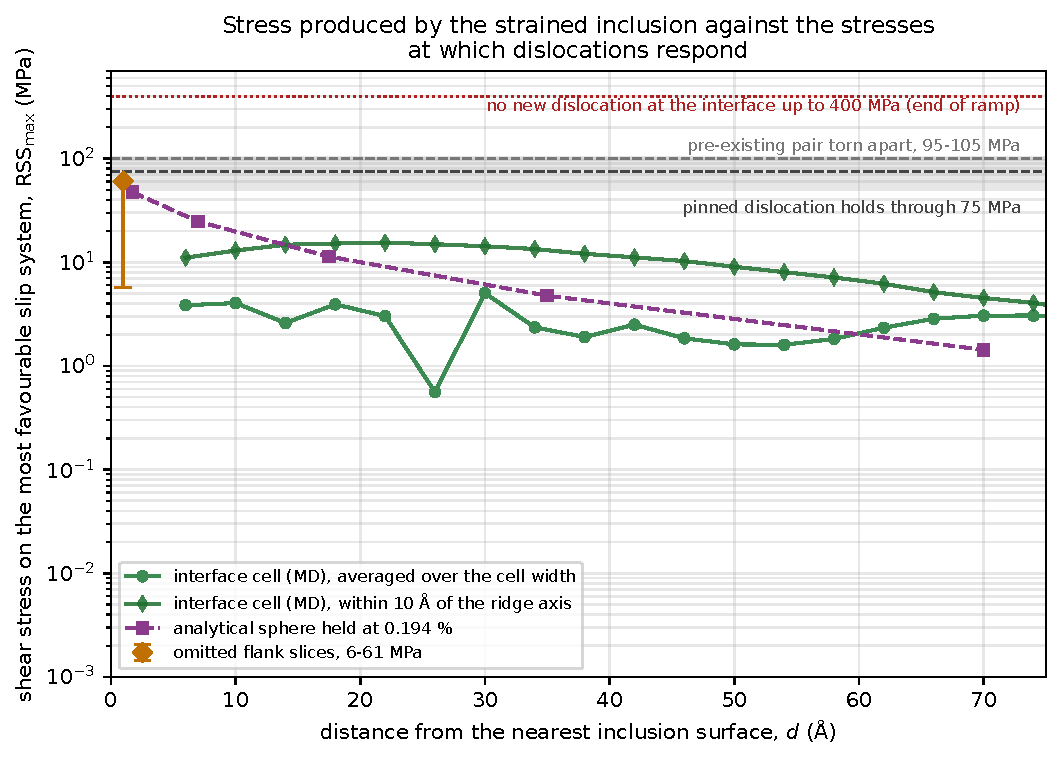
\includegraphics[width=0.9\linewidth]{fig_rss_vs_thresholds_en}
\caption{The stress produced by the strained inclusion against the stresses
at which dislocations respond: the shear stress resolved onto the most
favourable slip system, $\mathrm{RSS}_{\max}$, on a logarithmic scale,
against the distance $d$ from the nearest inclusion surface. Green circles:
the interface cell (91\,428 atoms) with the ridge held at 0.194\%, averaged
over the width of the cell; green diamonds: the same within 10~\AA{} of the
ridge axis; for the ridge $d=r-20$~\AA{} (the crest height). Purple squares:
the exact solution of Eshelby \cite{Eshelby1957} for a spherical inclusion
of radius $a=35$~\AA{} held at the same elongation in an infinite elastic
aluminium matrix ($\mu=26.5$~GPa, $\nu=0.347$, the volume-conserving
elongation of Eq.~(\ref{eq:eigenstrain}) with its axis at $45^{\circ}$ to
$z$, the same maximum over the twelve slip systems); for the sphere
$d=r-a$. Horizontal lines: the end of the ramp, 400~MPa, up to which no new
dislocation formed at the interface (dotted), and the stress at which the
pre-existing dislocation pair starts to move (95--105~MPa), both from
Section~\ref{sec:thresholds}; the shaded band, $75\pm22$~MPa, is the stress
withstood by the pinned dislocation of Section~\ref{sec:mobility} (the
applied 75~MPa, plus or minus the 22~MPa mutual stress of the pair, whose
sign is not resolved). The orange diamond marks the range spanned by the
omitted slices on the ridge flanks; it is not a measurement of the field.}
\label{fig:rss}
\end{figure}

\begin{figure}
\centering
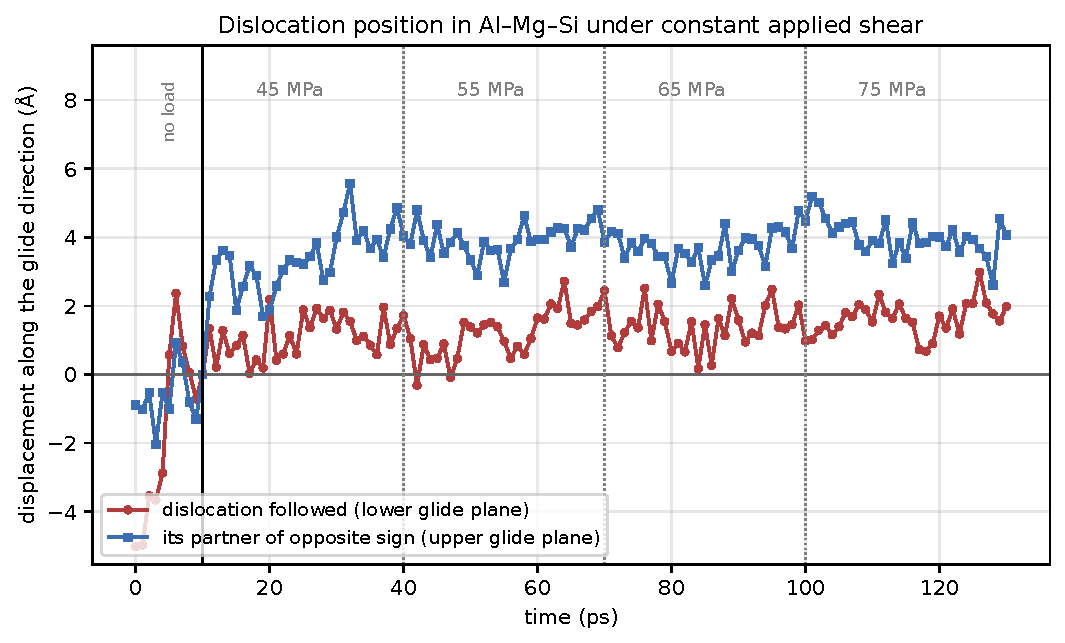
\includegraphics[width=0.9\linewidth]{fig_trajectories_en}
\caption{Position of the dislocation along its glide direction as a function
of time in the Al--Mg--Si cell under the staircase of constant applied shear
stresses (dotted lines: rung boundaries; the applied stress is written above
each rung; the displacement is measured from the position at the moment the load is
switched on, $t=10$~ps, after 10~ps without load). Red: the dislocation whose motion is followed (the
lower member of the pair); blue: its partner of opposite sign on the upper
glide plane. The dislocation oscillates about one position and does not
move: there is no plastic displacement at any of the four stress levels.
Over the whole loading history it advances 2.0~\AA{}, less than one Burgers
vector $b=2.86$~\AA{}, against a thermal oscillation of 0.6~\AA{}. The
partner takes up 4.1~\AA{} ($1.4\,b$) when the load is switched on and then
stops: over the remaining three rungs its position changes by less than its
thermal oscillation of 0.5~\AA{}. That single initial step is not sustained
glide.
}
\label{fig:traj}
\end{figure}

\subsection{Dislocation mobility and solute pinning in the alloy}
\label{sec:mobility}

The resistance that dissolved Mg and Si atoms oppose to dislocation motion
was measured in the alloy cell of Section~\ref{sec:loading}: no inclusion,
1.0~at.\% Mg and 0.6~at.\% Si substituted at random for aluminium, and one
pair of edge dislocations of opposite sign on glide planes 206~\AA{} apart,
loaded by a staircase of constant applied shear stresses of 45, 55, 65 and
75~MPa, 30~ps each. Figure~\ref{fig:traj} shows the position of the
dislocation whose motion is followed (the lower member of the pair) and of
its partner as a function of time. The dislocation does not glide. Over the
120~ps of loading it advances 2.0~\AA{}---less than one Burgers vector
$b=2.86$~\AA{}---against a thermal oscillation of 0.6~\AA{}; the
net displacements within the four rungs, 0.6, 1.6, $-1.5$ and 0.2~\AA{} at
45, 55, 65 and 75~MPa, are comparable to that oscillation and do not grow
with stress. The line oscillates about one position and remains held by the
solute atoms around it at every stress level. A velocity can of course be
fitted to each rung, but at these displacement-to-oscillation ratios
(all below 3) it would measure the oscillation and not a drift, and none is
quoted. What the trajectory does establish is a lower bound: the sampled
random configuration of Mg and Si atoms holds the dislocation against a
driving stress of at least 75~MPa. This exceeds the 15~MPa that the held ridge produces at its
surface (Section~\ref{sec:sigma_r}) by a factor of 5, and the 41~MPa
of the analytical sphere by a factor of 1.8. The two dislocations of the pair
exert a mutual stress of 22~MPa on each other, whose sign relative to the
applied shear is not resolved here, so the conservative reading of the bound
is $75\pm22$~MPa, with a lower edge of 53~MPa, which still exceeds both
amplitudes.
The bound also lies above the Labusch estimate $\tau_c\approx38$~MPa for
this solute content \cite{Labusch1970,Leyson2010}---the mean-field estimate
of the stress needed to drag a dislocation through a random distribution of
solute atoms---which is consistent with a locally stronger-than-average
arrangement of solutes in this single realization.

In the solute-free reference cell of the same geometry the dislocation moves
freely: its position wanders by up to about 20~\AA{} within individual
stress steps, and no trapping event occurs in the 130~ps trajectory. Within
this model, pinning by solute atoms is therefore the only obstacle to
dislocation motion represented in these cells. A quantitative law of
dislocation drag in pure aluminium could not be extracted from the same
geometry: without obstacles one member of the pair reaches the free surface
and is absorbed within the first stress step, and the excursions of the
remaining line are bounded by the residual field of the periodic dislocation
construction; the pinning observation in the alloy is therefore benchmarked
against the Labusch estimate rather than against a measured drag
coefficient. Because no depinning event occurs, the activation volume $V^{*}$ (the volume swept by a dislocation segment as it crosses an obstacle, which sets how strongly the glide rate responds to stress) cannot be extracted from these runs.
The value $V^{*}=70\,b^{3}$ reported by Soula et al.\ for Al--Mg--Si
processed by equal-channel angular pressing \cite{Soula2022JALCOM} is used
as the central case; because that material state differs from the present
one, the range $V^{*}=19$--$142\,b^{3}$ \cite{CaillardMartin2003} is used
only as a sensitivity range. The trajectory serves solely to bound the
obstacle strength from below. No Mg/Si clusters were constructed or identified. A second random
configuration, run only through the 45, 55 and 65~MPa rungs, was likewise
pinned at every rung it reached; the 75~MPa bound rests on the one
realization that completed the staircase.

\section{From local resolved shear to macroscopic creep}
\label{sec:bridge}

The results of Section~\ref{sec:results} bound what a strained inclusion can
do locally. To connect them with the macroscopic observation the question is
turned around: how large a stress around the inclusions would be needed to
raise the creep rate by the measured 25\%? The estimate that answers it has
three ingredients.

The first is the shape of the stress field. Outside a compact particle of
radius $a$ that is bonded to the matrix and strained, the elastic solution of
Eshelby \cite{Eshelby1957} gives a stress that falls off with distance $r$
from the particle centre as $(a/r)^{3}$. The resolved shear stress---the part
of the stress that pushes a dislocation (Section~\ref{sec:stress}), and hence
the only part that pushes a dislocation---is written in this scalar form as
$\tau(r)=\tau_m(a/r)^{3}$, with $\tau_m$ its value at the particle surface. In
a dilute dispersion with inclusion volume fraction $f$, the fraction of matrix
volume in which $|\tau|$ exceeds a given level $s$ is
$F(>s)=f\,(\tau_m/s-1)$ for $0<s<\tau_m$ (the volume of the particle itself
is subtracted), and the distribution of stress levels over the matrix volume
is given by the density $p(s)=-\mathrm{d}F/\mathrm{d}s=f\,\tau_m/s^{2}$.

The second is the response of dislocation glide to stress. At room
temperature dislocations pass obstacles by thermally activated jumps, and a
local stress $\tau$ changes the jump rate by the factor
$\exp(\pm V^{*}\tau/kT)$. Here $V^{*}$ is the activation volume of Section~\ref{sec:mobility}
\cite{CaillardMartin2003}. Because the stress around a particle
takes both signs, the two directions are weighted equally and the rate is
proportional to $\cosh(V^{*}\tau/kT)$.

The third is the averaging. The creep rate of the alloy is the rate averaged
over the matrix volume, so $\cosh(V^{*}\tau/kT)-1$ is integrated over the
density $p(s)$. The relative enhancement of the creep rate is
\begin{equation}
\frac{\langle\dot\varepsilon\rangle}{\dot\varepsilon_0}-1
 = f\,x_0\!\int_{0}^{x_0}\!\frac{\cosh u-1}{u^{2}}\,\mathrm{d}u
 = f\left[x_0\,\mathrm{Shi}(x_0)-(\cosh x_0-1)\right],
\label{eq:bridge}
\end{equation}
with $x_0=V^{*}\tau_m/kT$, where
$\mathrm{Shi}(x)=\int_0^x\sinh u\,\mathrm{d}u/u$ is the hyperbolic sine
integral. The integral is taken down to $s=0$, i.e.\ it assumes that the
stressed shells of neighbouring particles do not overlap; cutting it off where
they would (at $u_{\min}=f x_0$, where the shell of one particle reaches its
neighbours) lowers the predicted enhancement from 0.2500 to 0.2499 and raises
the required $\tau_m$ by about $0.01\%$ at every $V^{*}$ in
Table~\ref{tab:bridge}, so the tabulated values stand.
Equation~(\ref{eq:bridge}) is a model estimate of sensitivity, not an
extraction of the interface stress from the experiment: it describes the field
by a single amplitude $\tau_m$, weights positive and negative stresses
equally, and takes the spatial statistics of the $(a/r)^{3}$ field. It
matters that $\tau_m$ is the amplitude of the resolved shear at the particle
surface, not the full interface stress, of which only a part acts in any one
slip plane.

The inputs are the following. The temperature is 300~K. The inclusion content of the alloy is
0.35~wt\%, corresponding to a volume fraction $f=0.00246$, within the
0.1--0.3\% reported in Ref.~\cite{Friha2024JMMM}; Table~\ref{tab:bridge} is
evaluated at this value.
The activation volume is taken in the range $V^{*}=19$--$142\,b^{3}$, which
spans the values for aluminium alloys \cite{CaillardMartin2003}, with
$V^{*}=70\,b^{3}$ measured for Al--Mg--Si \cite{Soula2022JALCOM} as the
central case; no value of $V^{*}$ was extracted from the present simulations
(Section~\ref{sec:mobility}), so the range is a sensitivity range within the
model, not a measured input.

The output is Table~\ref{tab:bridge}. Its second column is obtained by
setting the left side of Eq.~(\ref{eq:bridge}) to 0.25 and solving for
$\tau_m$: 8.4--62.7~MPa across the range of $V^{*}$, the larger values at the
smaller activation volumes. Although the enhancement is proportional to $f$
at fixed $\tau_m$, the required $\tau_m$ is obtained by inverting a nonlinear
function and therefore does not scale as $1/f$: direct recalculation gives
9.8--73.3~MPa at $f=0.001$ and 8.1--60.3~MPa at $f=0.003$.

Three comparisons follow. If the 147~MPa of Ref.~\cite{Friha2024JMMM} were
the resolved shear stress acting on the dislocations, Eq.~(\ref{eq:bridge})
would predict enhancements from $6.8\times10^{2}$ to $2.7\times10^{46}$
(third column), at least $2.7\times10^{3}$ times the observed 0.25; 147~MPa
acting as a shear stress is incompatible with the observed enhancement. The
stress that an inclusion strained by 0.194\% actually produces is smaller.
For a bonded sphere held at that strain the exact solution \cite{Eshelby1957}
gives 41~MPa of resolved shear inside the particle and just outside it (Section~\ref{sec:sigma_r});
with this amplitude Eq.~(\ref{eq:bridge}) gives 0.045 at $V^{*}=19\,b^{3}$,
0.31 at $30\,b^{3}$ and values far above 0.25 at larger $V^{*}$ (fourth
column). The ridge of the interface cell, held at the same strain, produces
15~MPa of resolved shear just above its crest
(Section~\ref{sec:sigma_r}); with this amplitude the estimate gives
0.042 at $V^{*}=50\,b^{3}$ and 0.16 at $70\,b^{3}$, the
activation volume measured for Al--Mg--Si \cite{Soula2022JALCOM} (last
column). At a strain of 0.194\%, therefore, the stress around the inclusions
is of the order the estimate requires: the observed 0.25 is reproduced for
$V^{*}$ between about 30 and 75$\,b^{3}$, depending on which
of the two amplitudes is taken.

This is a consistency, not a confirmation, for three reasons. The estimate
is exponentially sensitive to the product $V^{*}\tau_m$: doubling $V^{*}$ at
fixed amplitude moves the prediction by two to four orders of magnitude, so
the agreement fixes little beyond the order of magnitude. The strain of
0.194\% is an input taken from the earlier estimate of the interface stress
\cite{Friha2024JMMM}, not a measured property of the inclusions; the
magnetostriction measured for bulk iron--aluminium alloys does not exceed
$10^{-4}$ \cite{Hall1959,BormioNunes2012}, twenty times less, and since the
stress is proportional to the strain an inclusion strained by $10^{-4}$ would
produce at most 2~MPa at its surface, for which Eq.~(\ref{eq:bridge}) gives
an enhancement below 0.4\% at every $V^{*}$ in the range. And the estimate
describes a field that exists while the inclusion is strained; it says
nothing about the tens of minutes for which the effect persists after the
field is removed (Section~\ref{sec:memory}). Whether the inclusions of this
alloy strain by 0.194\% in a field of 0.7~T is therefore the question on
which the elastic mechanism stands or falls, and it is an experimental one.

\begin{table}
\centering
\caption{The two-scale estimate, Eq.~(\ref{eq:bridge}), at $T=300$~K,
$f=0.00246$ and $b=2.8638$~\AA{}. Second column: the resolved
shear stress $\tau_m$ at the particle surface that reproduces the measured
$+25\%$ creep enhancement. The remaining columns give the enhancement
$\langle\dot\varepsilon\rangle/\dot\varepsilon_0-1$ that
Eq.~(\ref{eq:bridge}) predicts if $\tau_m$ were 147~MPa (the earlier
estimate), 41~MPa (the interior value of the analytical sphere held at 0.194\%, which
is also the amplitude of its inverse-cube far field; 41.45 unrounded) or 15~MPa (the maximum on the ridge axis in the interface
cell, 15.45 unrounded, Section~\ref{sec:sigma_r}). The observed value is 0.25.}
\label{tab:bridge}
\small
\begin{tabular}{lcccc}
\hline
$V^{*}$ & $\tau_m$ for $+25\%$ (MPa) & at 147~MPa & at 41~MPa & at 15~MPa \\
\hline
$19\,b^{3}$  & 62.7 & $6.8\times10^{2}$  & 0.045 & 0.004 \\
$30\,b^{3}$  & 39.7 & $3.9\times10^{6}$  & 0.31 & 0.010 \\
$50\,b^{3}$  & 23.8 & $3.9\times10^{13}$ & 17 & 0.042 \\
$70\,b^{3}$  & 17.0 & $4.8\times10^{20}$ & $1.2\times10^{3}$ & 0.16 \\
$100\,b^{3}$ & 11.9 & $2.4\times10^{31}$ & $9.3\times10^{5}$ & 1.2 \\
$142\,b^{3}$ & 8.4  & $2.7\times10^{46}$ & $1.2\times10^{10}$ & 31 \\
\hline
\end{tabular}
\end{table}

\section{Discussion}
\label{sec:discussion}

\subsection{Three stresses, and the identity of the magnetic phase}
\label{sec:phase}

Three stresses appear in this paper and must be kept apart. The first is the
147~MPa of Ref.~\cite{Friha2024JMMM}. It is an estimate of the stress at the
inclusion surface, obtained from the field through an empirical coefficient;
it is not a measured stress, not a resolved shear stress on any slip plane,
and not a result of the present calculations. If it were the shear stress on
a slip plane it would exceed the 95--105~MPa at which the lower
partner of the dislocation pair of Section~\ref{sec:thresholds} breaks away,
so the loaded cells cannot test it by comparison with a threshold; what they
test is whether a strained inclusion produces anything of that order in the
matrix. The second is what
a bonded elastic inclusion strained by 0.194\% supplies. The exact solution
for a bonded sphere \cite{Eshelby1957}---no sliding at the interface: the
atoms on both sides interact through the same potential, and no artificial
constraint is applied there---gives 41~MPa of resolved shear inside the particle,
falling as $(a/r)^{3}$ outside (Fig.~\ref{fig:rss}). The third is the field
measured in the cell for the same strain held fixed
(Section~\ref{sec:sigma_r}): 15~MPa of resolved shear just above
the crest of the ridge, falling within 80~\AA{} to $2.5\pm0.5$~MPa, the resolution of the
calculation; averaged over the width of the cell the peak is
5.0~MPa, because the ridge occupies less than half of that
width. The second and the third stress are of one order and together
bracket the amplitude entered in Eq.~(\ref{eq:bridge}). The first exceeds
them by a factor of 3.6--10 because $E\varepsilon$ is the stress of a rod held
at that strain, not of an inclusion embedded in a matrix that deforms with
it.

A separate difficulty concerns the phase itself. In the batch studied, X-ray
diffraction identifies the inclusions as Al$_{13}$Fe$_4$ (written
Fe$_4$Al$_{13}$ in Ref.~\cite{Friha2024JMMM}; the form Al$_{13}$Fe$_4$ is
used throughout here), and the magnetization of the samples shows a
hysteresis loop, i.e.\ the inclusions contain a ferromagnetic constituent
\cite{Friha2024JMMM}; earlier work in the same series gives the composition
of the inclusions as Fe$_x$Al$_{1-x}$ with $x=86$--$87$~at.\%
\cite{Skvortsov2019JAP,Nikolaev2025SciRep}. Stoichiometric Al$_{13}$Fe$_4$,
however, shows no magnetic order down to 2~K---neither in its magnetization
nor in M\"ossbauer spectra, which probe the magnetic state of the iron atoms
directly \cite{Avers2025Crystals,Albedah2015Mossbauer}: the
ideal compound does not magnetize and cannot change shape through
magnetization (which does not, by itself, guarantee a strictly zero strain of
any other origin). The measured ferromagnetism of the inclusions therefore
belongs not to the ideal Al$_{13}$Fe$_4$ lattice but to some other
constituent of them---iron-rich regions of the kind noted in
Refs.~\cite{Skvortsov2019JAP,Nikolaev2025SciRep}, for example---and it is the
strain of that constituent under field that matters for the mechanism. That
strain has not been measured for the inclusions of this alloy; the $10^{-4}$
used above is the largest value reported for bulk iron--aluminium alloys
\cite{Hall1959,BormioNunes2012}. The simulation cell represents the
inclusion by Al$_{13}$Fe$_4$ as the phase identified in this batch, with a
known structure \cite{Liu2024CIF}; the strain applied to it is taken as a
given. Measuring the strain of the actual inclusions under field is the
decisive experimental step.

\subsection{Why the mechanism cannot be simulated directly, and what MD can
measure instead}

A dislocation behaves as a line under tension. To bow it through a stressed
region of size $L$ the stress must exceed about $\mu b/L$, where $\mu$ is
the shear modulus and $b$ the Burgers vector \cite{CaillardMartin2003}. If
the whole claimed 147~MPa acted as resolved shear stress---the assumption most
favourable to the mechanism---this criterion gives $L\approx52$~nm (about
$180\,b$), i.e.\ a cell of some $2\times10^{8}$ atoms once the surrounding
matrix is included, against the roughly $10^{5}$ atoms of the cells used here.
At 41~MPa the corresponding size is about 0.2~$\mu$m, and at 15~MPa
about 0.5~$\mu$m. The mechanism therefore cannot be simulated directly at the
atomic scale. What molecular dynamics can supply is the quantities that a
description on the larger scale consumes: the stress at the interface and its
decay with distance (Section~\ref{sec:sigma_r}), the stresses at which
dislocations are set in motion or created
(Sections~\ref{sec:thresholds}--\ref{sec:mobility}), and, through
Eq.~(\ref{eq:bridge}), a check that the whole chain is self-consistent.

\subsection{The memory protocol}
\label{sec:memory}

In the experiments the field is absent during creep. The sample is held in the
field for 30~min, the field is removed, and only then is the load applied
\cite{Skvortsov2019PSS,Nikolaev2025SciRep}; what is measured is a memory of
the exposure.
Whatever the field does must therefore persist for tens of minutes after it
is gone. An elastic strain of the inclusion cannot: once the field is removed
the inclusion returns to its original shape and the stress around it
disappears within nanoseconds. The present calculations contain an inclusion held at its strain while the
matrix relaxes (the interface cell), one relaxed from it (the free cell) and
loaded cells with the inclusion free (unstrained) or held (unstrained and strained); none of them represents the
state of the material after the field has been removed. What could last
for tens of minutes is a slow rearrangement of atoms---for instance of the Mg
and Si atoms that pin the dislocations (Section~\ref{sec:mobility})---set in
motion while the field acted. Such a rearrangement has not been established
here. Supporting it would require the thermal history and the vacancy content
of the samples, an estimate of the diffusion rates, and a separate calculation
in which the field is switched on, held, switched off and the load then
applied. It is therefore stated here as one hypothesis that can be tested,
not as a result.

\subsection{Limitations}
\label{sec:limitations}

Two features of the geometry limit the transfer of these numbers to a real
particle. In the cell the inclusion is a ridge---a bar of half-elliptic cross
section running the full length of the cell along $y$
(Section~\ref{sec:cell})---rather than a compact particle. The stress outside
such a bar falls off with distance more slowly than the $(a/r)^{3}$ of a
compact particle, and its reach---some 30~\AA{} at full strength, 80~\AA{} in all
(Section~\ref{sec:sigma_r})---is set by the cross section of the ridge; it is a property of this cell, not of a micron-sized inclusion, whose
field would extend correspondingly further. Equation~(\ref{eq:bridge}) takes
its spatial statistics from the three-dimensional solution for a compact
particle and its amplitude either from that solution (41~MPa) or from the
ridge cell (15~MPa); the two differ by a factor of about
2.7, which is the effect of the geometry and is carried
through Table~\ref{tab:bridge} as the difference between its last two
columns. A two-dimensional elastic calculation for the ridge alone, with
the same strain and elastic constants but in an unbounded matrix of the same
stiffness, gives 20~MPa at the ridge surface falling to 5~MPa
within 10~\AA{}; the atomistic ridge, held rigid on its rigid layer, gives a
smaller surface value and a flatter profile. The atomistic and the continuum
description of the ridge thus agree in magnitude, and the difference from
the sphere is geometric, not an artefact of the cell.

The interatomic potential \cite{Jelinek2012} was chosen for its coverage of
Al, Fe, Mg and Si; how well it reproduces the Al/Al$_{13}$Fe$_4$ interface,
the stress needed to create dislocations, the structure of the dislocation
core and the pinning by Mg and Si has not been checked independently here, so
the absolute thresholds should be regarded as model-dependent. The residual
mismatch between the two lattices is the same in the control and strained
cells and cancels to first order in their difference; nonlinear relaxation may
prevent exact cancellation.

The thresholds of Section~\ref{sec:thresholds} are observations in a single
cell, with one set of initial atomic velocities and one loading rate; they
should be repeated with independent sets of starting velocities and at least a
second rate. The pinning result rests on two random arrangements of Mg and Si atoms,
only one of which completed the staircase, and one set of starting
velocities each; a statistical pinning threshold
would require three to five independent arrangements and velocity sets. This
is also why the pinning is reported as an observation and no activation
volume is extracted from it. The thermostat---the algorithm that holds the
cell at 300~K---acts on all mobile atoms and may itself influence the
thresholds and the temperature rise when the two dislocations meet and
annihilate; the dynamic stage should
be repeated either with the thermostat switched off after the temperature has
been established, or with it acting only on the atoms at the cell boundaries.

The field is represented only mechanically, as a strain of the inclusion.
Mechanisms in which the field acts directly on the dislocation or on the
obstacle, as in the theories of Refs.~\cite{Alshits2003,Molotskii2000}, are
outside the scope of the calculation. It is worth noting that the changes of
barrier height invoked by those theories, 0.01--0.1~eV, correspond through
$V^{*}\Delta\tau$ to 0.97--9.7~MPa at $V^{*}=70\,b^{3}$, and to
0.48--35.9~MPa over the whole range of $V^{*}$---overlapping the stresses
found here rather than coinciding with them. The stresses themselves are
computed from the atomic forces and positions (the virial expression
\cite{Thompson2022LAMMPS}) averaged over slices 4~\AA{} thick parallel to the
interface; this is an approximation whose resolution, after the six stress
components have been averaged over each slice, is $2.5\pm0.5$~MPa. Finally,
Eq.~(\ref{eq:bridge}) is a separate model relating a local stress to a change
of creep rate; it does not remove the dependence of the MD thresholds
themselves on the loading rate.

\section{Conclusions}
\label{sec:conclusions}

The stress that a strained inclusion produces in the matrix was computed in
an Al/Al$_{13}$Fe$_4$ interface cell of 91\,428 atoms for an elongation of
the inclusion by 0.194\% along the field direction at constant volume, the
strain corresponding to the earlier estimate of 147~MPa, with the inclusion
held at that strain. The resolved shear stress in the matrix reaches
15~MPa just above the inclusion and falls to the far-field level
of $2.5\pm0.5$~MPa within 80~\AA{}; averaged over the width of the cell the
peak is 5.0~MPa. The analytical solution for a compact particle
held at the same strain gives 41~MPa inside it, falling as the inverse
cube of the distance, so that for a micron-sized inclusion the same field
extends over a fraction of a micron. An inclusion that is not held relaxes
most of the strain.

In the loaded cells, a pre-existing pair of dislocations next to the ridge
is torn apart at an applied shear of 95--105~MPa with the inclusion free to relax; with the inclusion held, the strained and the unstrained cell coincide within one frame of the ramp, 9~MPa, at every stage; no new dislocation forms at the interface up to the end of the ramp at 400~MPa in the unstrained cell; and a random
arrangement of Mg and Si atoms holds a dislocation through 75~MPa. The first picoseconds of every ramp, at zero applied stress, answer the question whether the field of the strained ridge alone moves a dislocation placed next to it: the same partner moves in the same way with the ridge strained and unstrained, driven by the coherency field of the interface, not by the strain of the ridge.
These values are specific to the cells, the loading rate and the potential
and are not material constants.

The two-scale estimate, Eq.~(\ref{eq:bridge}), requires a resolved shear
stress of 8.4--62.7~MPa at the inclusion surface to raise the creep rate by
25\% at $f=0.00246$ and $V^{*}=19$--$142\,b^{3}$. The computed amplitudes,
41~MPa for the particle and 15~MPa for the ridge, reproduce the
observed enhancement for $V^{*}$ of 30--75$\,b^{3}$, a range
that contains the value measured for Al--Mg--Si; 147~MPa acting as resolved
shear would exceed the observed enhancement by a factor of at least
$2.7\times10^{3}$. The elastic mechanism is therefore quantitatively viable
if, and only if, the inclusions strain by about 0.2\% in the field: the
magnetostriction measured for bulk iron--aluminium alloys is twenty times
smaller and would give an enhancement below 0.4\%.

Because the field is off during the creep test, whatever it does must persist
for tens of minutes; an elastic strain cannot, and a slow rearrangement of
atoms is indicated as the remaining possibility---a hypothesis not tested by
the present calculations. The decisive next steps are the identification of
the ferromagnetic constituent of the inclusions, a direct measurement of their
strain under field, and a calculation in which the field is switched on, held,
switched off and the load then applied.

\section*{CRediT authorship contribution statement}
\textbf{I.~Mikhailovskiy:} Methodology, Software, Investigation, Formal
analysis, Visualization, Writing -- original draft.
\textbf{D.~Pshonkin:} Conceptualization, Resources, Supervision,
Writing -- review \& editing.

\section*{Data availability}
The structure generators, LAMMPS inputs, analysis code and the records behind
every number in this paper are in the public repository
\url{https://github.com/iluuua/magnetostriction-plasticity-bounds}. Each
figure and table is drawn from a JSON record written by one analysis script:
the stress profiles of Fig.~\ref{fig:sigma} and the atomistic curves of
Fig.~\ref{fig:rss} (\path{stageG10_field_profile.py}), the retained fraction
of the imposed strain (\path{stageG12_eigenstrain_retention.py}), the
analytical sphere (\path{stageG8_eshelby3d.py}) and the two-dimensional
solution for the ridge (\path{stageG17_ridge_continuum.py}),
Table~\ref{tab:bridge} (\path{stageG5_two_scale_bridge.py}), the dislocation
trajectories of Fig.~\ref{fig:traj} and the pinning bound
(\path{stageG6_vstar_analysis.py}, \path{stageG7_pinning_stats.py}), and the
onsets of Section~\ref{sec:thresholds} (\path{stageG2_depinning.py}). The two minimised interface cells
from which the stress field is measured are included with the code
(\path{data/stageG4_clean}); the renders of Figs.~\ref{fig:cell} and
\ref{fig:loading} are produced by \path{stageG14_render_cells.py}.

\section*{Declaration of competing interest}
The authors declare no competing financial interests.

\bibliographystyle{elsarticle-num}
\bibliography{references}

\end{document}
